
\section*{1D analysis of topological states}
In order to have a chiral Hamiltonian I will choose the orientation of the dipoles in a way, such that the chirality remains. This will be done for each lattice configuration separately, i.e. the dipoles depend on the lattice geometry.\\
In order to make the achievement of chirality more feasible I only consider nearest neighbour interactions. When talking of chirality the chirality of the matrix $U$, defined above, is in mind. Recall that
\begin{align*}
    U_{n,m}&=
        -\frac{\partial^2 V_{n,m}(\mathbf{r}_{nm})}{\partial\mathbf{r}_{nm}^2}\quad\text{if}\:n\neq m\\
    U_{n,n} &= \sum_{j;\,j\neq n}\frac{\partial^2 V_{n,j}(\mathbf{r}_{nj})}{\partial\mathbf{r}_{nj}^2}
\end{align*}
Chirality implies that all couplings between sites on the same sublattice vanish. The nearest neighbour restriction already assures that couplings between different sites of the same sublattice vanish. Left is thus only the onsite potential due to the taylor expansion of the dipole dipole potential. The aim is now to choose the orientaiton of the dipoles in such a way that the sum in $U_{n,n}$ is equal to zero.\\ Be aware that so far I didn't write explicitely the dependence of $U$ from the direction of atom movement $x$, $y$. Hence $U_{n,m}$, $U_{n,n}$ are themselves two times two matrixes $(U_{n,m}^{\alpha,\beta})_{\alpha,\beta\in\{x,y\}}$ and the Hamilonian expressed explicitely with respect to the $x$, $y$-phonon modes reads
\begin{align*}
    H &= \sum_{n,\alpha} \omega\,a_{n,\alpha}^\dagger a_{n,\alpha} +\frac{2}{m\omega}\, \sum_{n,m,\alpha,\beta} U^{\alpha,\beta}_{n,m}\,a_{n,\alpha}^\dagger a_{m,\beta}    
\end{align*}
The terms with $a_{n,\alpha}^\dagger a_{n,\alpha}$ can thus be eliminiated by redefining the trap frequency.
\begin{align*}
    \omega_\alpha=\omega+\frac{2}{m\omega}\,U^{\alpha,\alpha}_{n,n}
\end{align*}
% Because on the borders $U_{n,n}^{\alpha,\alpha}$ is different from the bulk values, the trap potential for the atoms on the boundary have to be altered to compensate this shift. As I tested in the simulation the existence of separated energies in the bulk band gabs breaks down when the Hamiltonian on the border is different from the bulk.

The terms coupling the two directions of phonon modes on the same side can not be internalized by another quantity. Here the degrees of freedom related to the dipole orientation are exploited to tune the $U_{n,n}^{x,y}$ values to zero, as mentioned above. Because of the nearest neighbour nature of the consideration only two distances play a role, the intracell distance $\mathbf{r}_I$ and the intercell distance $\mathbf{r}_O$. 
\begin{align*}
    U_{n,n}^{x,y}= \frac{\partial^2 V(\mathbf{r}_{I})}{\partial {r}_{I,x}\partial r_{I,y}}+\frac{\partial^2 V(\mathbf{r}_{O})}{\partial {r}_{O,x}\partial r_{O,y}}
\end{align*}
The dipoles are then chosen in such a way that this sum vanishes. For open boundary conditions the values of $U_{n,n}^{\alpha,\beta}$ at the borders are different from the bulk values. In the case of $\alpha=\beta$ the difference can be compensated by changed trap frequencies at the boundary. For the $xy$ coupling this is not possible and the interaction due to both neighboring atoms has to made zero individually such that $x$- and $y$-modes are completely decoupled from each other. \\\\
The topologically non-trivial phase actually breaks down, when those border-terms are not eliminated. This is confirmed by simulations. It might be, at first, counter intuitive that reducing the effect of an open border is decremental to the observation of edge states. It makes, however perfect sense, when remembering that those boundary terms in our case destroy the chiral symmetry. It seems to be necessary for the bulk-boundary condition to hold that not only the momentum space Hamiltonian with periodic boundary conditions has to satisfy chiral symmetry but also the real space Hamiltonian with open boundary conditions. Otherwise one could choose the Hamiltonian describing the border in a completely arbitrary manner and still observe edge states, what would be quite a strong statement.\\\\
What one observes is that, if the same direction edge coupling is kept in, no separated energies in the bulk gaps arise. At the other hand if only the boundary terms, coupling the two phonon directions, remain and $U_{n,n}^{\alpha,\alpha}$ is completely absorbed into the trap frequencies separated energies inside the bulk energy gaps can be observed. These separated energies, however, are not located at zero and converge for the atom number going to infinity to a non-zero value, what makes them non-topological. 



\subsection*{Aligned dipoles in plane}
I consider a geometry with two sublattices repeating itself in the $x$-axis and separeted by the distance $h$ from each other into the $y$-axis. Different configurations of this geometry are realized by moving the sublattices against each other in the $x$-direction. I consider an even amount of lattice, with $N$ atoms in each sublattice. The $n$th atom of each sublattice $A$ and $B$ takes the position.
\begin{align*}
    \mathbf{r}^A_n&=n\cdot a \,\mathbf{e}_x\\
    \mathbf{r}^B_n&=n\cdot a\, \mathbf{e}_x + b\,\mathbf{e}_x+ h\,\mathbf{e}_y,
\end{align*}
where $a$ is the lattice constant, and the parameters $b$ and $h$ can be chosen to realize different lattice configurations with the restriction that $b$ and $h$ have to be chosen in a way, such that the nearest neighbor restriction makes sense. 
For any $b$-value it is possible to find $h$ and the dipole moment $\mathbf{d}$ in a way that fulfils the above conditions.\\\\
% By contemplating the spectrum in dependence of the parameter $b$ we find energy state that are well separated from the bulk energy \figref{fig:non_chiral_edge_spectrum}. But the separated energy values converge to a non-zero value, when the number of atoms goes to infinity. But this would be necessary for proper topological edge states. I assume this discrepancy occurs because, as I constructed the dipole moment, the components of the Hamiltonian related to the border are non vanishing. Only the bulk Hamiltonian obeys chiral symmetry. It makes of course sense that the chirality is not only required for the momentum space Hamiltonian with periodic boundary conditions but also for the real space Hamiltonian. In order for the bulk boundary correspondence to hold it seems to be necessary that the real space Hamiltonian satisfies the same symmetries as the momentum space Hamiltonian. Seems reasonable.\\\\
% Fortunately it is still possible to set 

% \begin{figure}
%     \centering
%     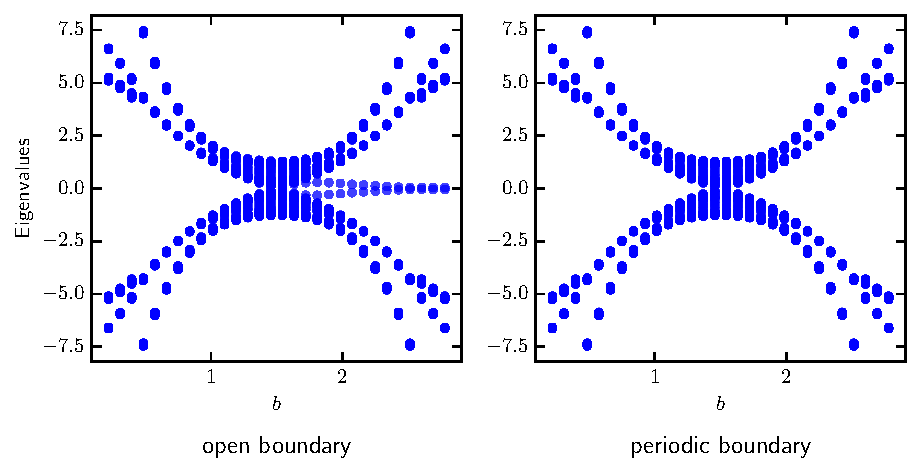
\includegraphics[scale=0.9]{pictures/aligned_dipole_in_plane_sheer_spectrum_h1.1_a3.pdf}
%     \caption{\textbf{Spectrum of almost chiral-symmetric Hamiltonian.}}
%     \label{fig:non_chiral_edge_spectrum}
% \end{figure} 



\begin{figure}[H]
    \centering
    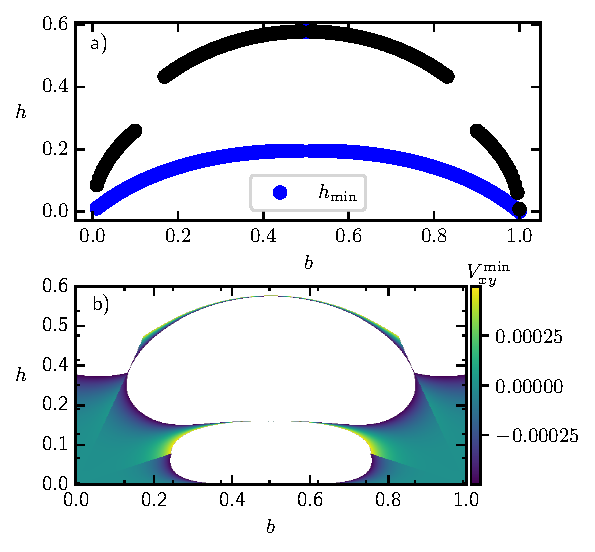
\includegraphics[]{pictures/aligned_dipoles_in_plane_sheer.pdf}
    \caption{\textbf{Optimal $h$ for chiral symmetry.} In \textbf{a)} The $h$ values are depicted which decouple $x$- and $y$-phonons. Those values were determined numerically by computing roots of $V_xy(h)$. A grid of $h$ values as initial guesses for the root algorithm was taken to have a better chance of finding all roots. In \textbf{b)} $V_xy(b,h)$ is drawn for reference. Larger values of the function have been omitted to make the pattern of small coupling values more visible.}
    \label{fig:h_for_chirality}
\end{figure} 


\begin{figure}[H]
    \centering
    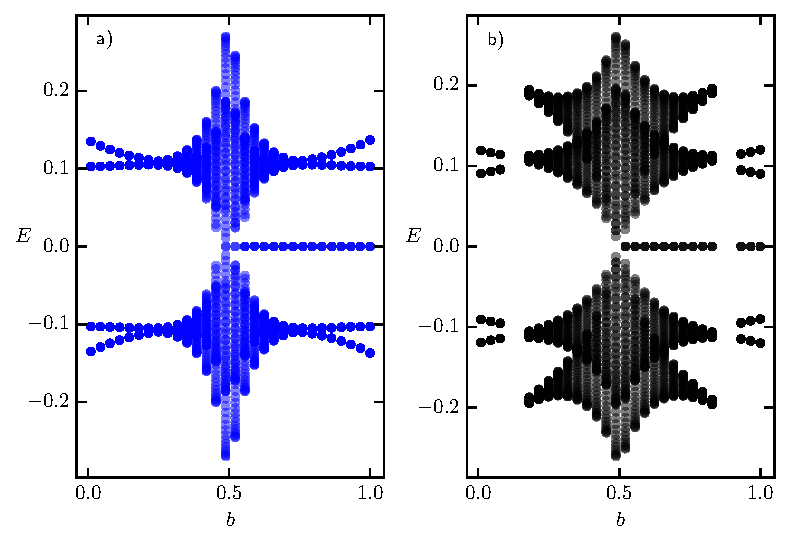
\includegraphics[]{pictures/aligned_dipoles_in_plane_sheer_spectrum_chrial.pdf}
    \caption{\textbf{Energy spectrum for the chiral Hamiltonian.}The diagram was created with the parameter $a=1$. Blue and black colors depict the Energy spectrum for the $h$ values picked from the blue and black curves in \figref{fig:h_for_chirality} respectively.}
\end{figure} 
\begin{figure}[H]
    \centering
    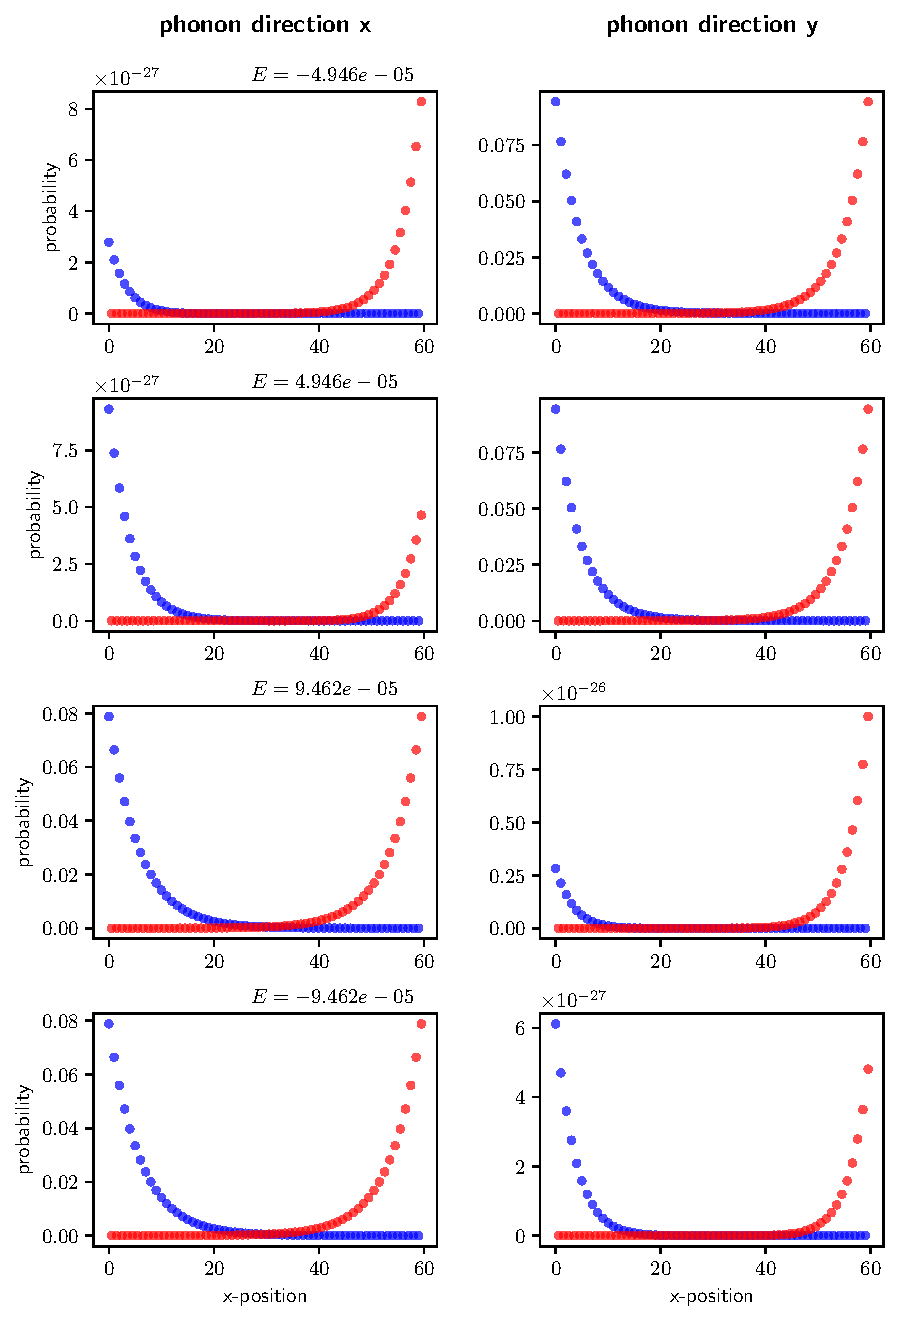
\includegraphics[]{pictures/ads_top_states_b0.51.pdf}
    \caption{\textbf{Edge states}. The figure shows the decay of edge states with the four energies with the smallest absolute value. Each row depicts one energy state. Drawn in blue are the excitations of sublattice A, while the excitation of sublattice B is shown in red.}
\end{figure} 
\begin{figure}[H]
    \centering
    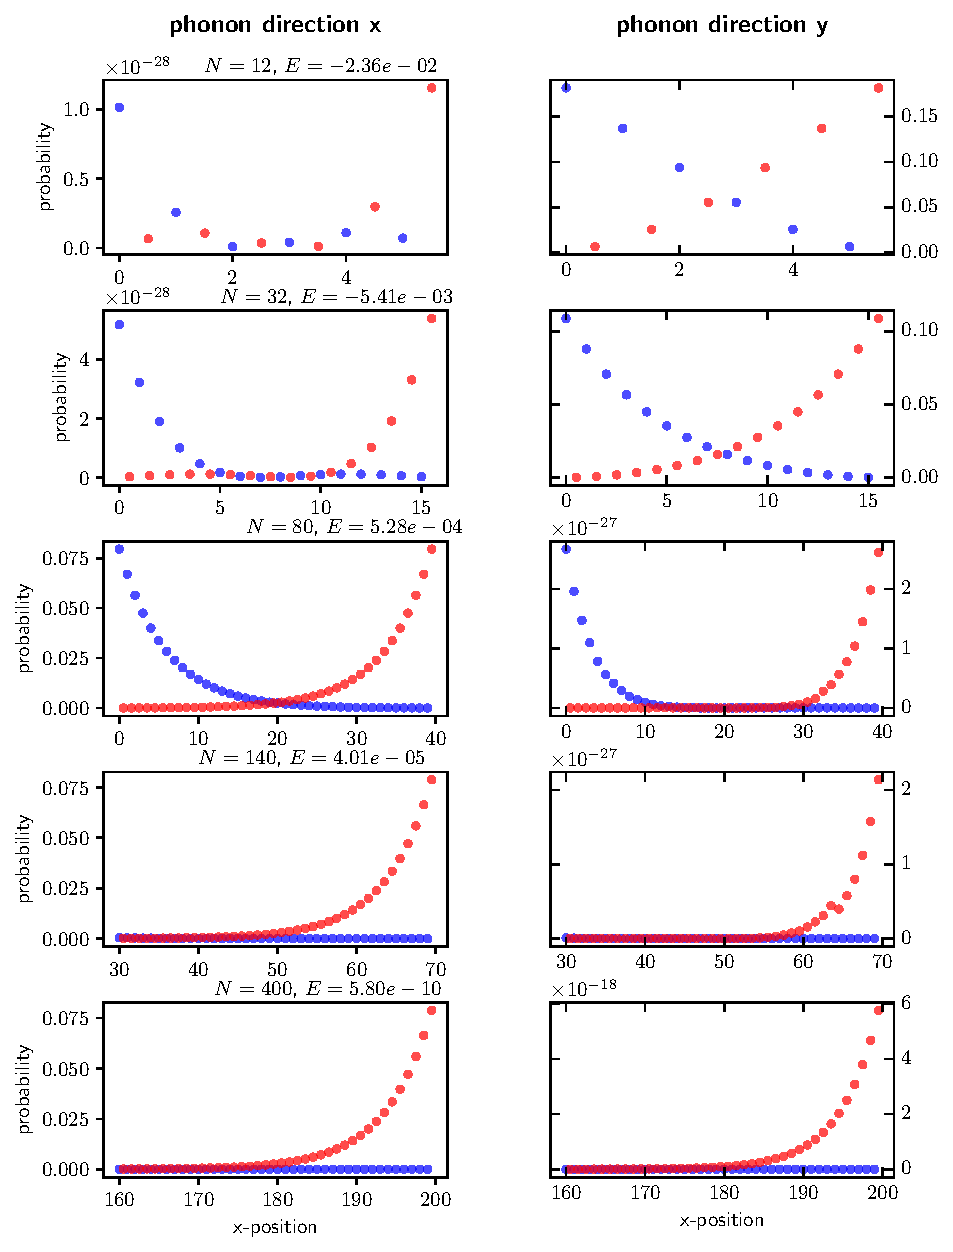
\includegraphics[]{pictures/ads_states_for_chain_lengths.pdf}
    \caption{\textbf{Decay of energy for topological states with atom number.}. In each row the eigenstate for the energy with smallest absolute value is plotted. Blue and red show again the excitations of sublattice A and B respectively. When moving down in the rows of the figure the atom number of the system is increased. It shows that with increasing atom number the energy of the topological decays. What also can be observed. That the decay-length of the excitations when moving away from the edges does not change with particle number.}
\end{figure} 
\begin{figure}
    \centering
    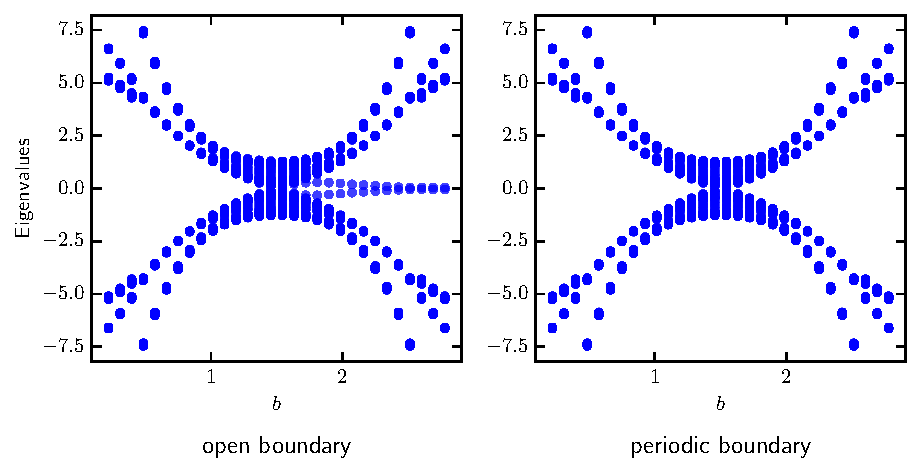
\includegraphics[scale=0.9]{pictures/aligned_dipole_in_plane_sheer_spectrum_h1.1_a3.pdf}
\end{figure} 
\begin{figure}
    \centering
    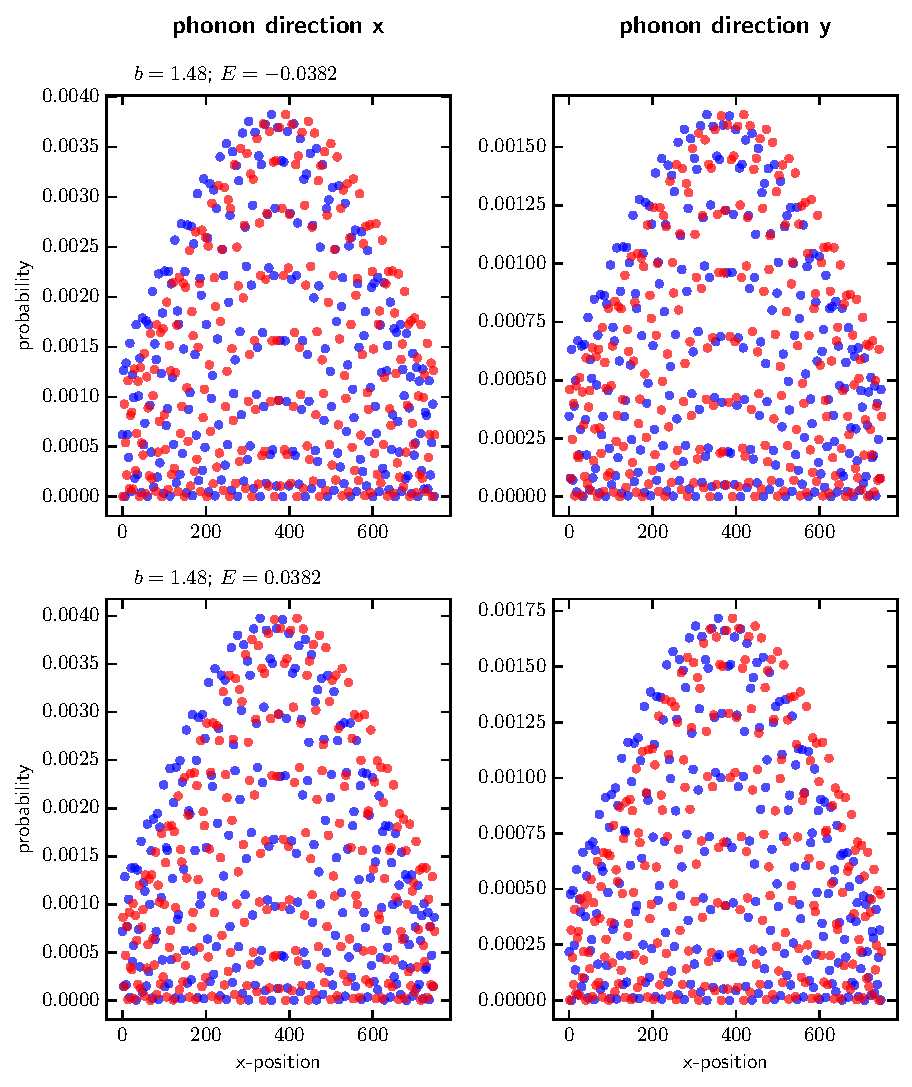
\includegraphics[scale=0.85]{pictures/aligned_dipoles_in_plane_sheer_h1.1_a3_eigenvecs0.pdf}
\end{figure} 
\begin{figure}
    \centering
    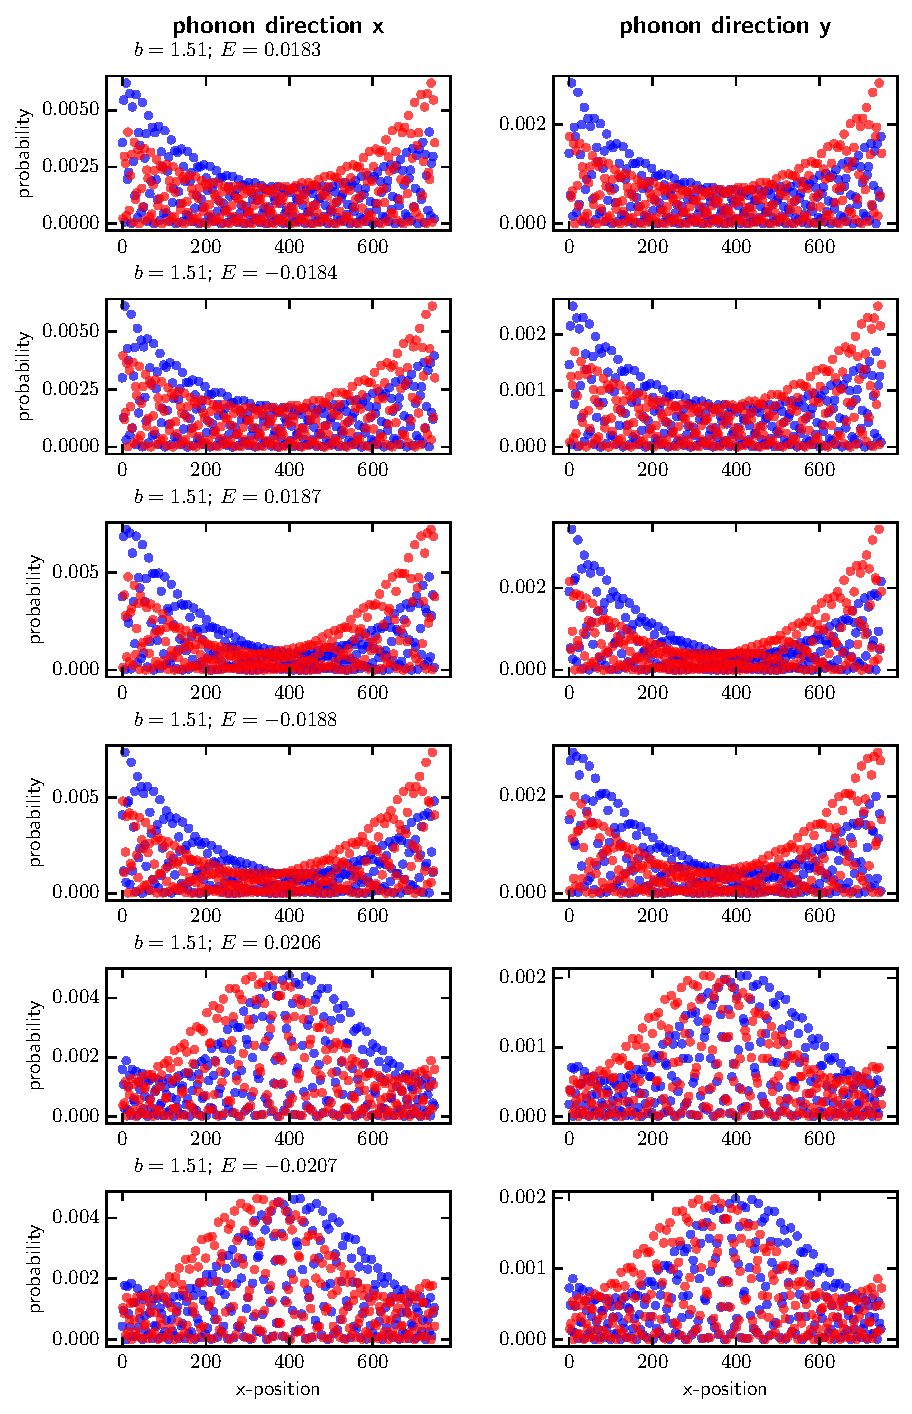
\includegraphics[]{pictures/aligned_dipoles_in_plane_sheer_h1.1_a3_eigenvecs1.pdf}
\end{figure}
\begin{figure}
    \centering
    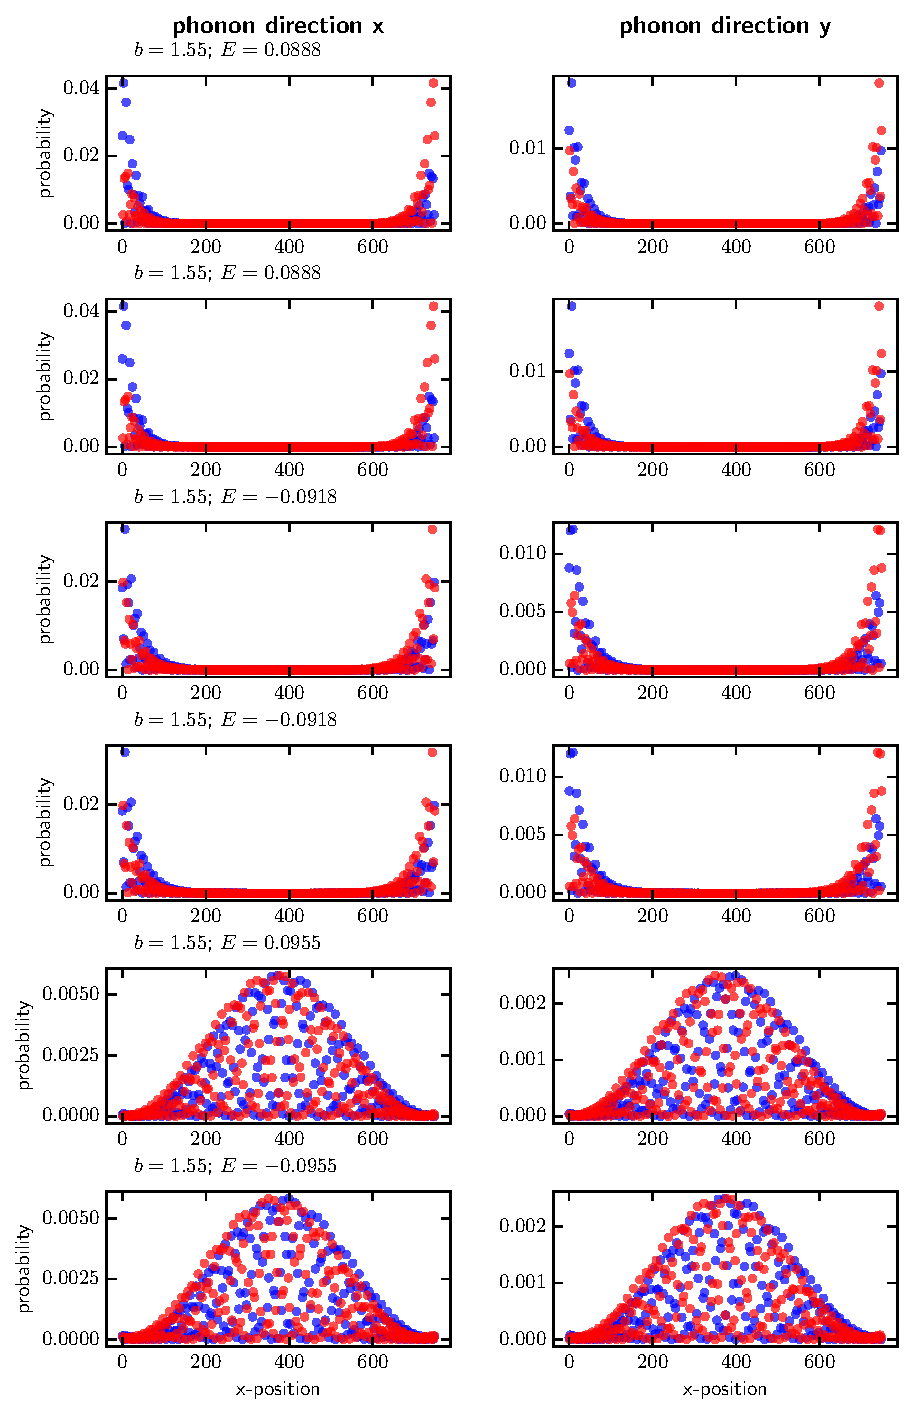
\includegraphics[]{pictures/aligned_dipoles_in_plane_sheer_h1.1_a3_eigenvecs2.pdf}
\end{figure}

\begin{figure}
    \centering
    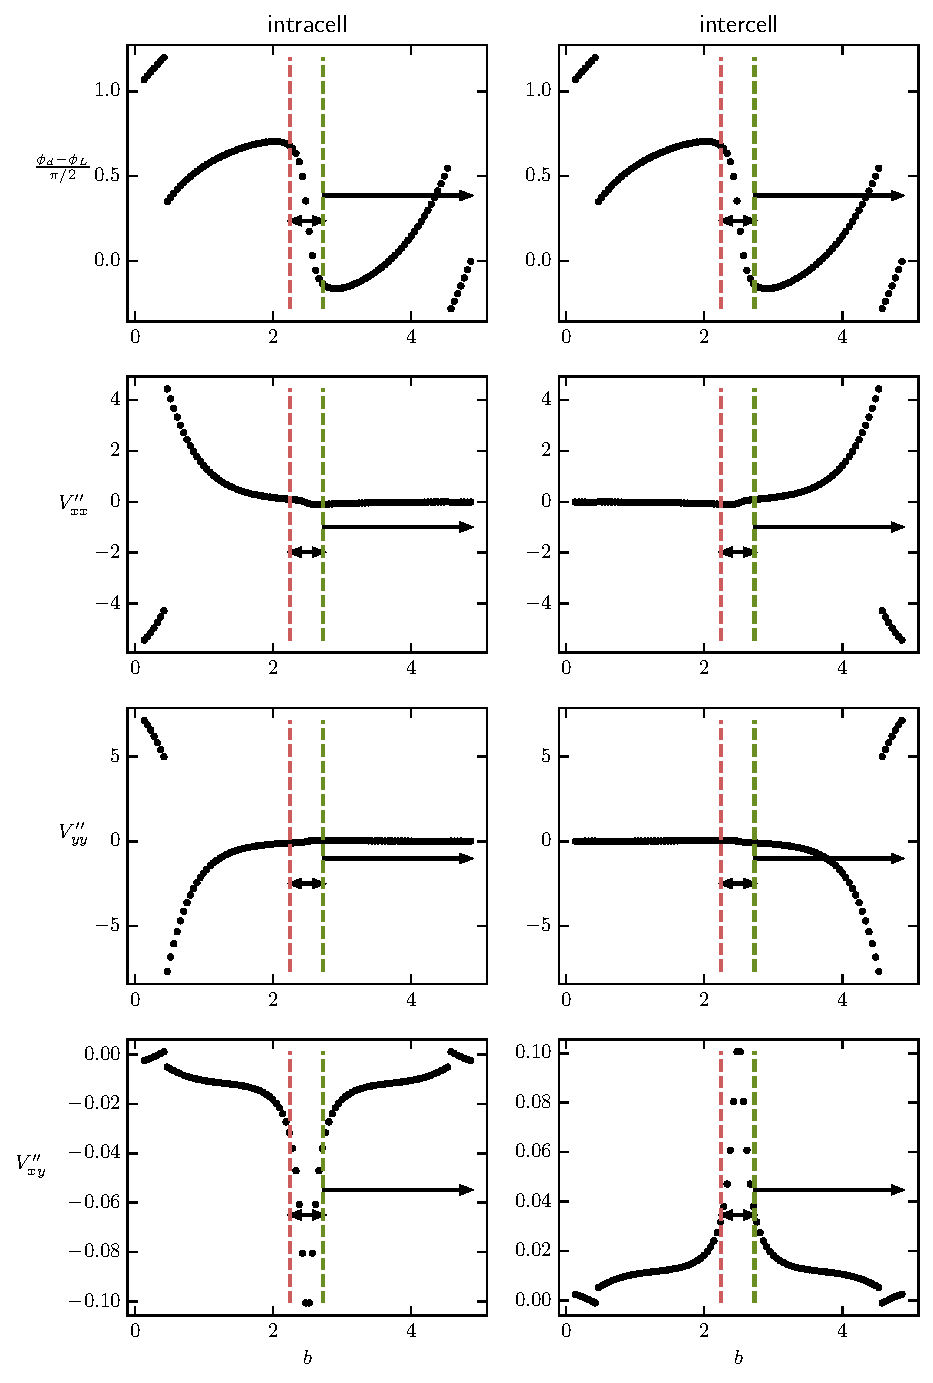
\includegraphics[]{pictures/aligned_dipoles_in_plane_orientation_sheer_h1.1_a5.pdf}
    \caption{The diagram was created with the parameters $a=5$, $h=1.1$. Between the red and the olive dashed line, i.e. bewteen $b$-values of $2.25$-$2.73$ the winding number is 1, whereas right to the olive dashed line the winding number is 2.}
\end{figure} 
\begin{figure}
    \centering
    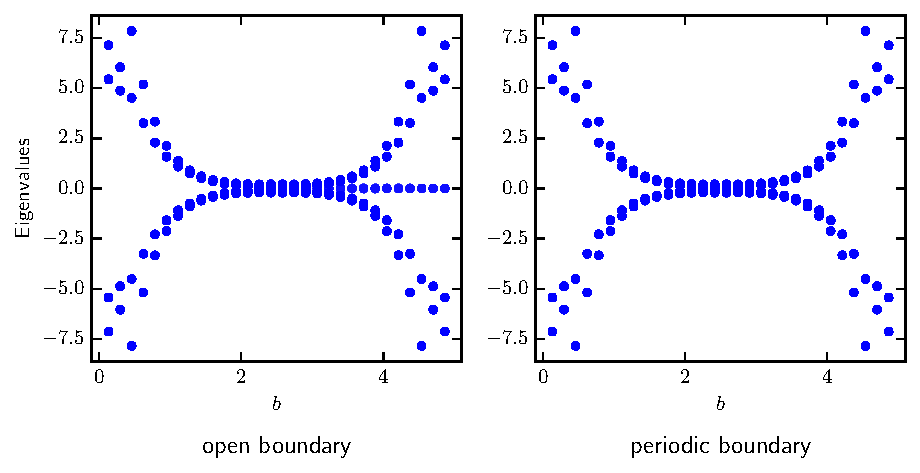
\includegraphics[scale=0.9]{pictures/aligned_dipole_in_plane_sheer_spectrum_h1.1_a5.pdf}
\end{figure} 
\begin{figure}
    \centering
    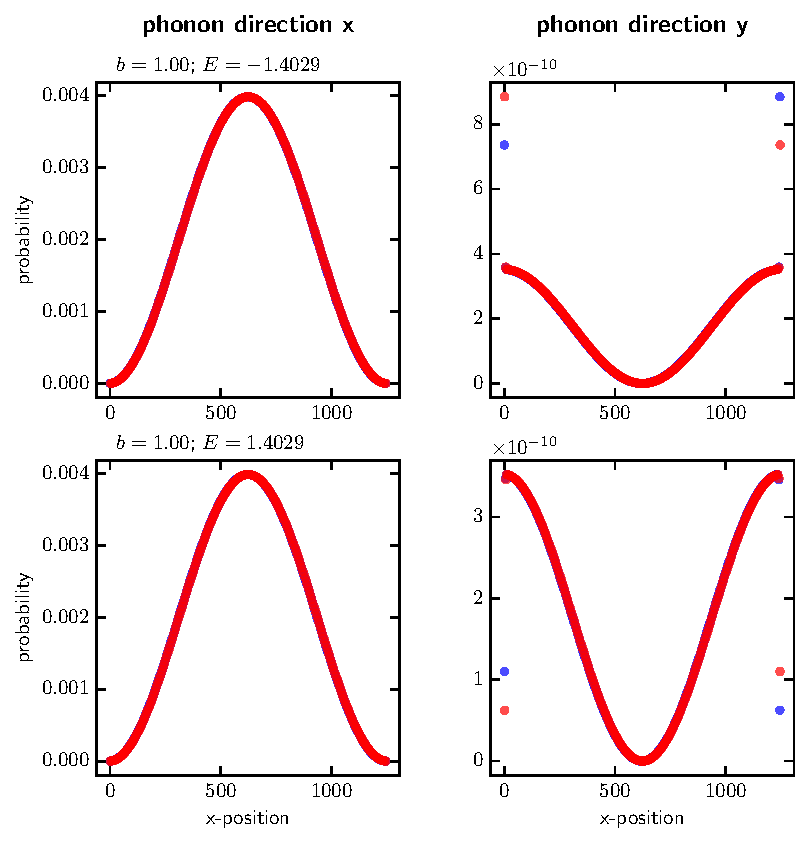
\includegraphics[]{pictures/aligned_dipoles_in_plane_sheer_h1.1_a5_eigenvecs0.pdf}
\end{figure} 
\begin{figure}
    \centering
    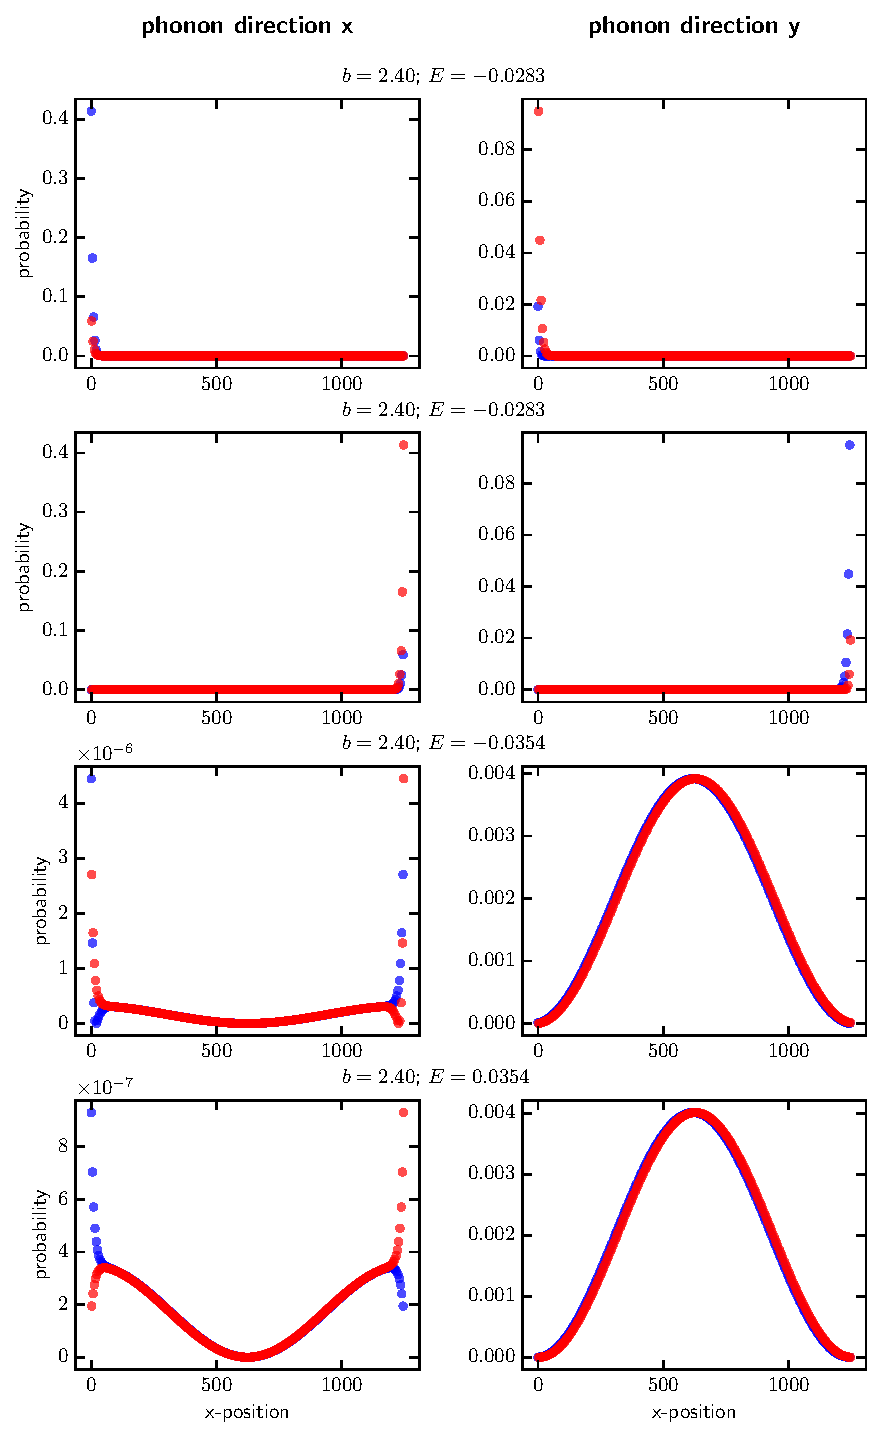
\includegraphics[]{pictures/aligned_dipoles_in_plane_sheer_h1.1_a5_eigenvecs1.pdf}
\end{figure}
\begin{figure}
    \centering
    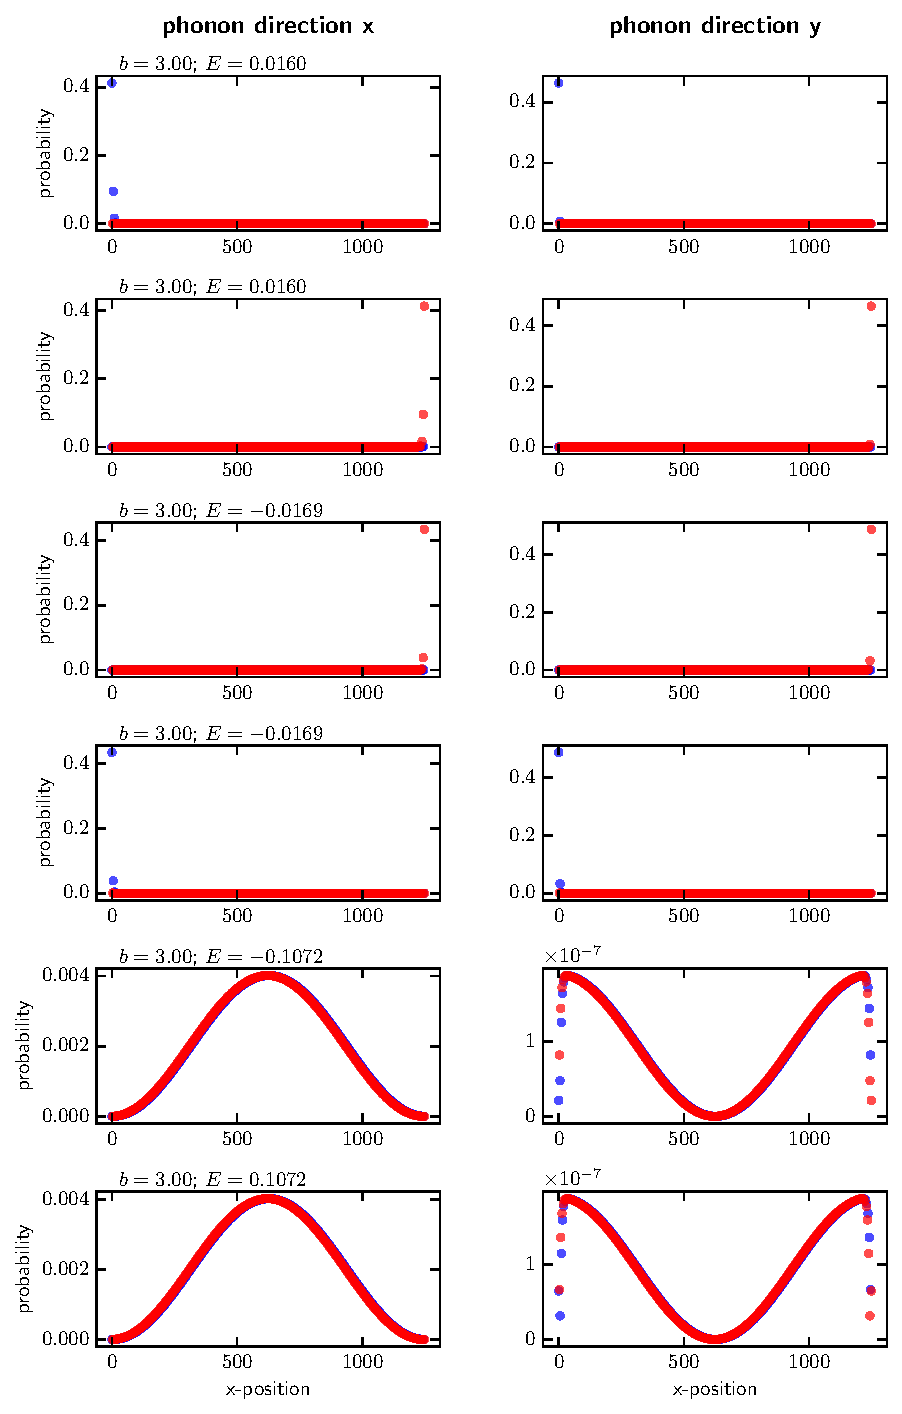
\includegraphics[]{pictures/aligned_dipoles_in_plane_sheer_h1.1_a5_eigenvecs2.pdf}
\end{figure}

\subsection*{Out of plane dipoles}
First I will allow the dipoles to point out of the $xy$-plane in which the one dimensional chain will reside. I restrict the dipoles to the following form in order to have easier calcualtions.
\begin{align*}
    \mathbf{d}_1= \begin{pmatrix}
        d_{1,x}\\
        0\\
        \sqrt{-d_{1,x}^2}
    \end{pmatrix},\quad
    \mathbf{d}_2= \begin{pmatrix}
        0\\
        d_{2,y}\\
        \sqrt{-d_{2,y}^2}
    \end{pmatrix}
\end{align*}
\begin{figure}[H]
    \centering
    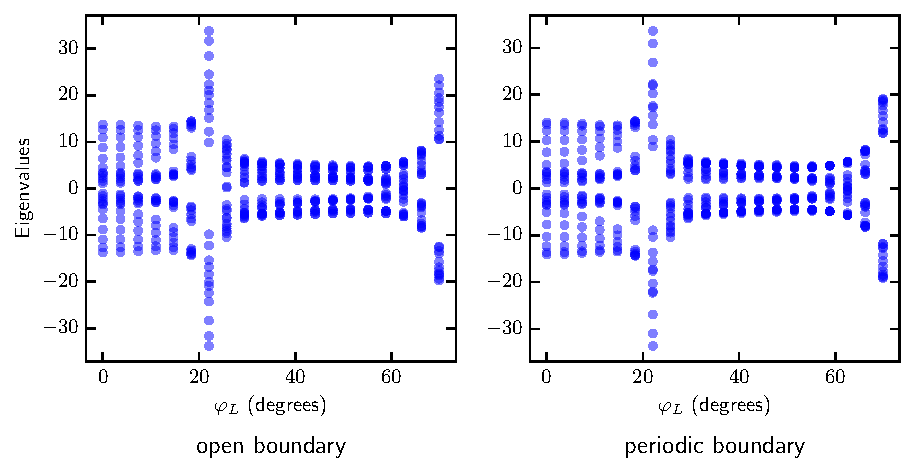
\includegraphics[]{pictures/out_of_plane_dipole_orientation_zigzag.pdf}
\end{figure}
\begin{figure}[H]
    \centering
    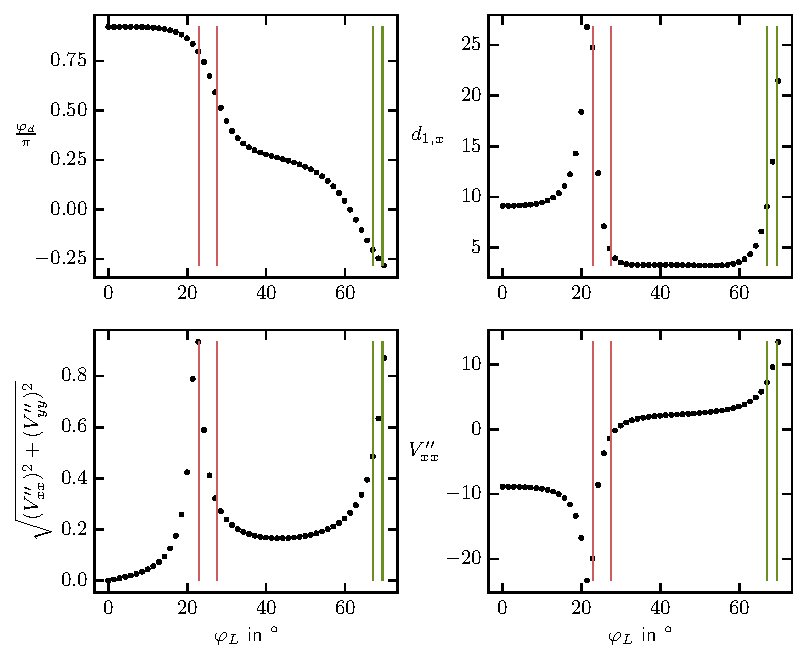
\includegraphics[]{pictures/dipole_orientation_off_plane.pdf}
    \caption{The occurance of topological states is signaled by the vertical lines. Between the two red as well as between the two green lines topological states can be found.}
\end{figure}%
As chain I consider a zig-zag chain with sublattice vector $\mathbf{a}_S$ and lattice vector $\mathbf{a}_L$.
\begin{align*}
    \mathbf{a}_S = \begin{pmatrix}
        c\\
        \epsilon
    \end{pmatrix},\quad\mathbf{a}_L = \begin{pmatrix}
        c+1\\
        0
    \end{pmatrix}
\end{align*}
For nearest neighbour interaction the condition that lets the momentum space Hamiltonian be chiral under periodic boudary conditions reads
\begin{align*}
    0&\overset{!}{=}V''_{xy}(\mathbf{a}_S)+V''_{xy}(\mathbf{a}_S-\mathbf{a}_L)\\
    V''_{xy}(\mathbf{r}_0)&\vcentcolon=\frac{\partial^2 V}{\partial r_x\partial r_y}(\mathbf{r}_0)
\end{align*}

With the particular dipole configuration, introduced above, the derived interaction takes the form
\begin{align*}
    V''_{xy}(\mathbf{r})&=d_{1,x}d_{2,y}\,\left( \frac{12}{r^5}-105\,\frac{r_x^2r_y^2}{r^9} \right)+15\,\sqrt{1-d_{1,x}^2}\,\sqrt{1-d_{2,y}^2}\,\frac{r_xr_y}{r^7}\\
    V''_{\alpha\alpha}(\mathbf{r})&=d_{1,x}d_{2,y}\,\left( 45\,\frac{r_xr_y}{r^7} - 105\,r_\alpha^2\,\frac{r_xr_y}{r^9} \right)+\sqrt{1-d_{1,x}^2}\,\sqrt{1-d_{2,y}^2}\,\left( -\frac{3}{r^5}+15\,\frac{r_\alpha^2}{r^7} \right)
\end{align*}


\subsection*{In plane dipole orientation}
As a next step I restrict the dipoles to the $xy$-plane seperate the magnitude of the dipole projected onto the plane from the occurance of topological states. In this scenario I investigate the properties of the dipole restriction of the following form.
\begin{align*}
    \mathbf{d}_1= \begin{pmatrix}
        d_{1,x}\\
        d_{1,y}\\
        0
    \end{pmatrix},\quad
    \mathbf{d}_2= \begin{pmatrix}
        d_2\\
        0\\
        0
    \end{pmatrix}
\end{align*}
For this configuration the interaction takes to From
\begin{align*}
    V''_{xy}(\mathbf{r})&=d_{1,x}d_2\,\left( 45\,\frac{r_xr_y}{r^7}-105\,\frac{r_x^3r_y}{r^9} \right)+ d_{1,y}d_2\,\left( \frac{12}{r^5}-105\,\frac{r_x^2r_y^2}{r^9} \right)\\
    V''_{\alpha\alpha}(\mathbf{r})&=d_{1,x}d_2\,\left[ -\frac{3+\delta_{\alpha,x}}{r^5}+\frac{15}{r^7}\,\left( r_x^2 + 2\,r_\alpha r_x+r_\alpha^2+2\delta_{\alpha,x}\,r_x^2\right) -105\,\frac{r_x^2\,r_\alpha^2}{r^9} \right]\\
    &+ d_{1,y}d_2\,\left[ \frac{15}{r^7}\,\left( r_xr_y + 2\delta_{\alpha,x}\,r_xr_y\right)-105\,\frac{r_\alpha^2r_xr_y}{r^9} \right]
\end{align*}

\begin{figure}[H]
    \centering
    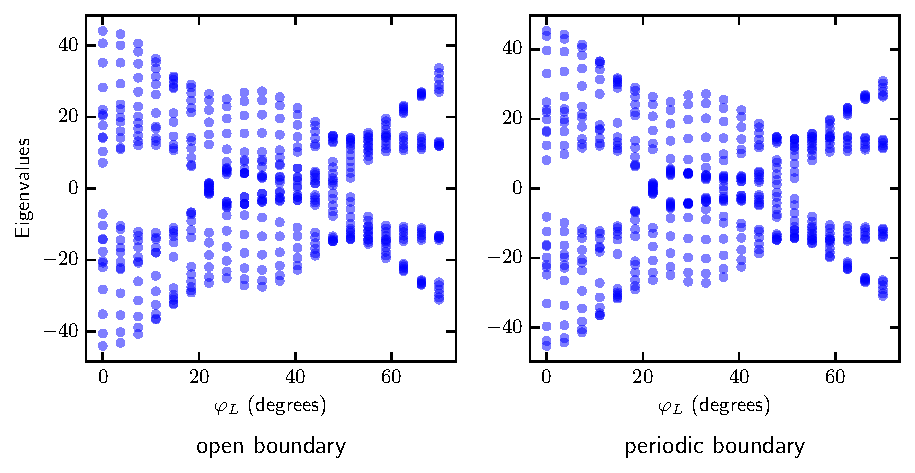
\includegraphics[]{pictures/inplane_dipole_orientation_zigzag.pdf}
\end{figure} 
\begin{figure}[H]
    \centering
    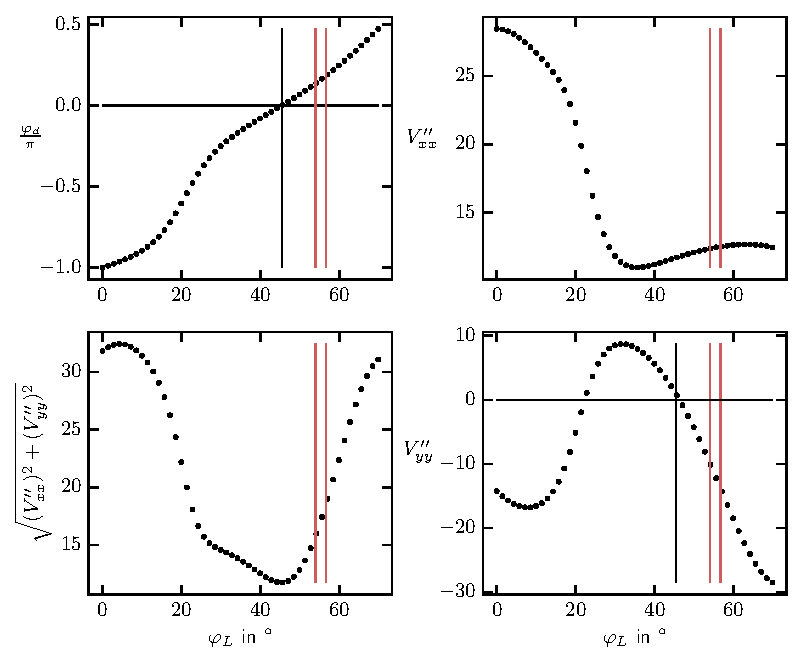
\includegraphics[]{pictures/dipole_orientation_in_plain.pdf}
    \caption{Topological states can again be found in the angle range between the two red vertical lines.}
\end{figure}

\subsection*{1D hexagonal chain}
In this chapter I consider a chain with equal spacing $r$ between the atoms where the angle $\varphi$ is changed in a manner, such that the first layer of a 2D hexagonal lattice is reached. Because of the one dimensionality of the chain the unit cell contains four atoms (A, B, C, D).
\begin{align*}
    \mathbf{a}_L&=\begin{pmatrix}
        2r\,(1+\cos\varphi_L)\\0
    \end{pmatrix}\quad\mathbf{a}_B=\begin{pmatrix}
        r\cos\varphi_L\\r\sin\varphi_L
    \end{pmatrix}\\
    \mathbf{a}_C&=\begin{pmatrix}
        r\,(1+\cos\varphi_L)\\r\sin\varphi_L
    \end{pmatrix}\quad\mathbf{a}_D=\begin{pmatrix}
        r\,(1+2\cos\varphi_L)\\0
    \end{pmatrix}
\end{align*}

\begin{figure}[H]
    \centering
    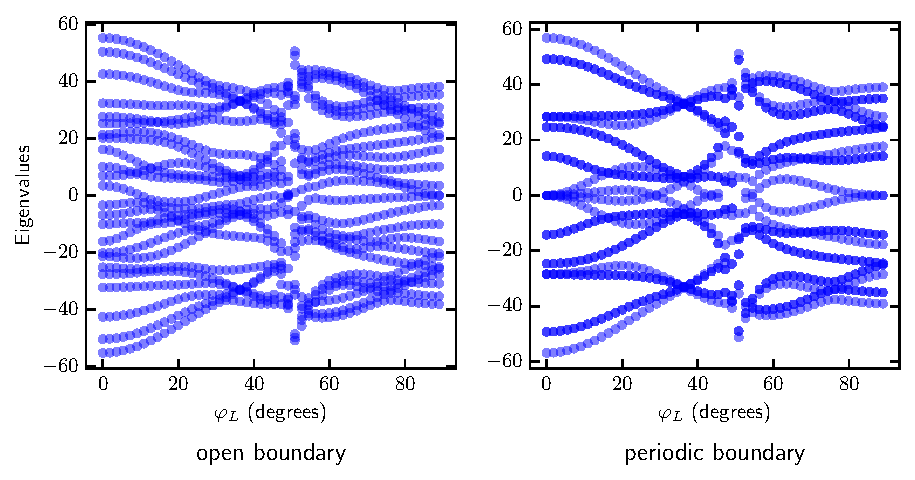
\includegraphics[]{pictures/in_plane_dipole_orientation_hex1D.pdf}
\end{figure} 
\begin{figure}[H]
    \centering
    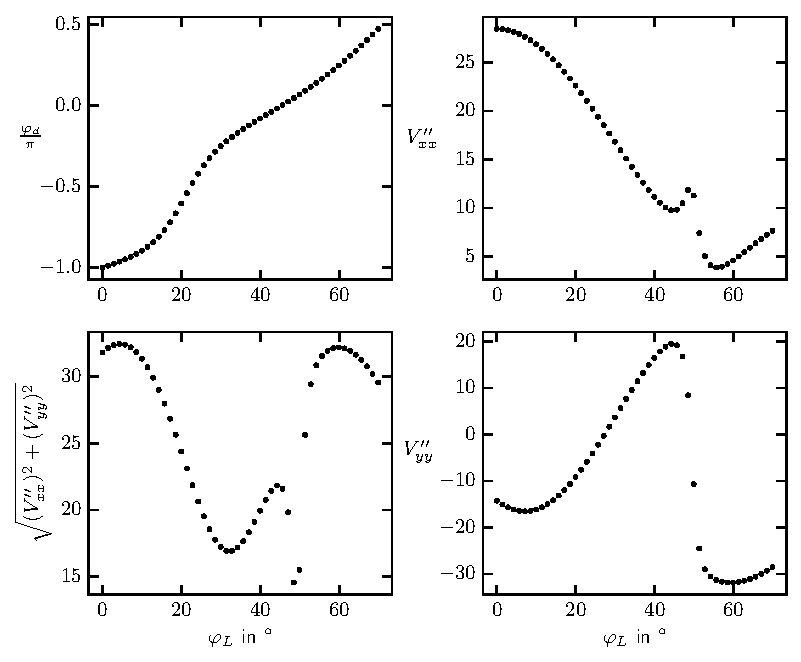
\includegraphics[]{pictures/dipole_orientation_in_plane_hex1D.pdf}
    \caption{In this configuration with equal spacing between the atoms no topological states occur.}
\end{figure}

\section{Aligned dipoles in plane}
\begin{figure}[H]
    \centering
    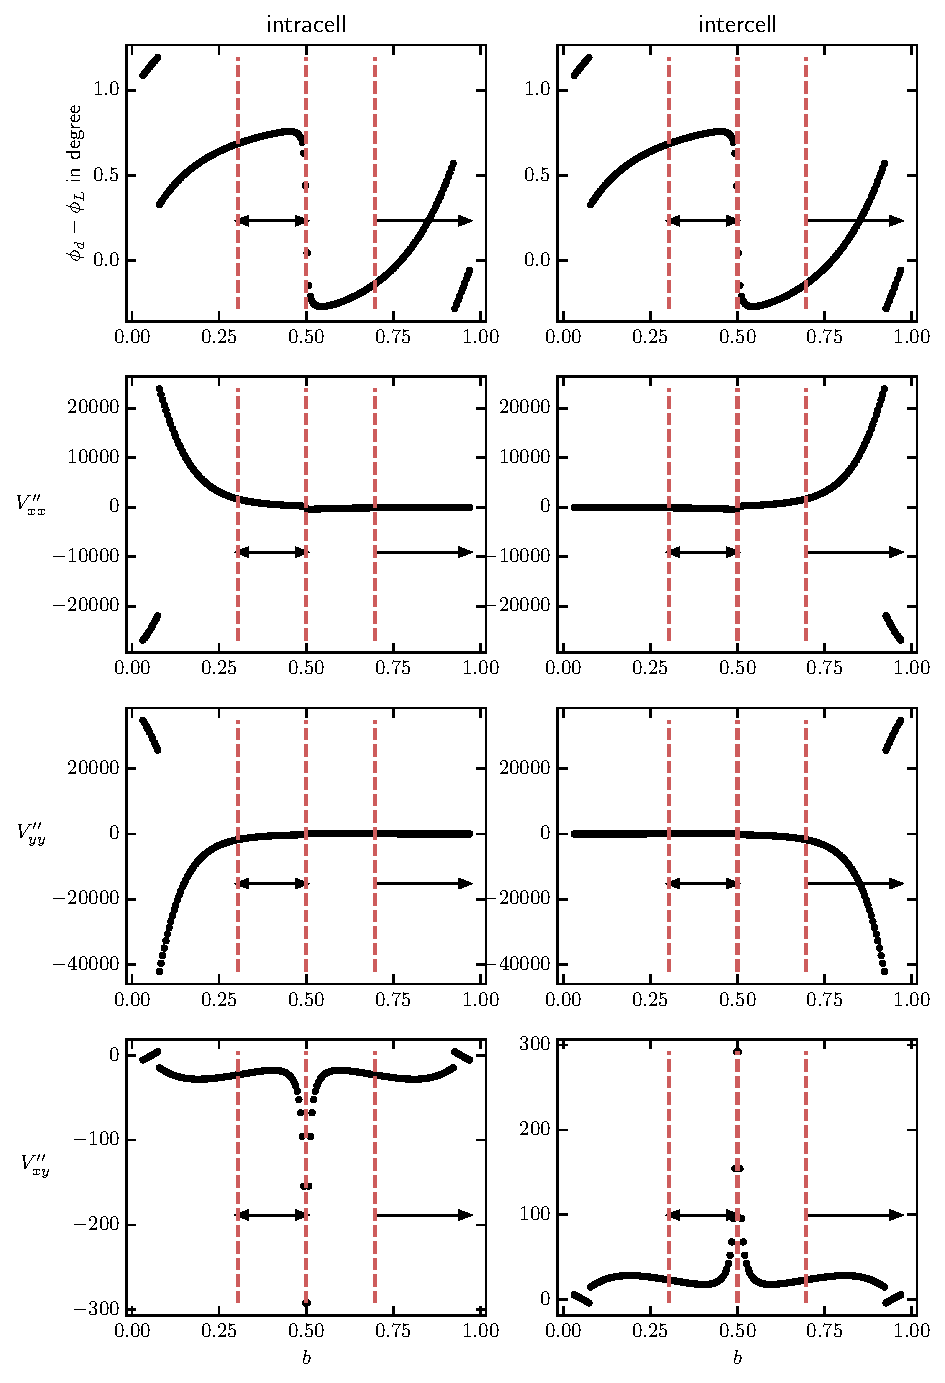
\includegraphics[]{pictures/aligned_dipoles_in_plane_zigzag_h0.2.pdf}
\end{figure} 
\begin{figure}[H]
    \centering
    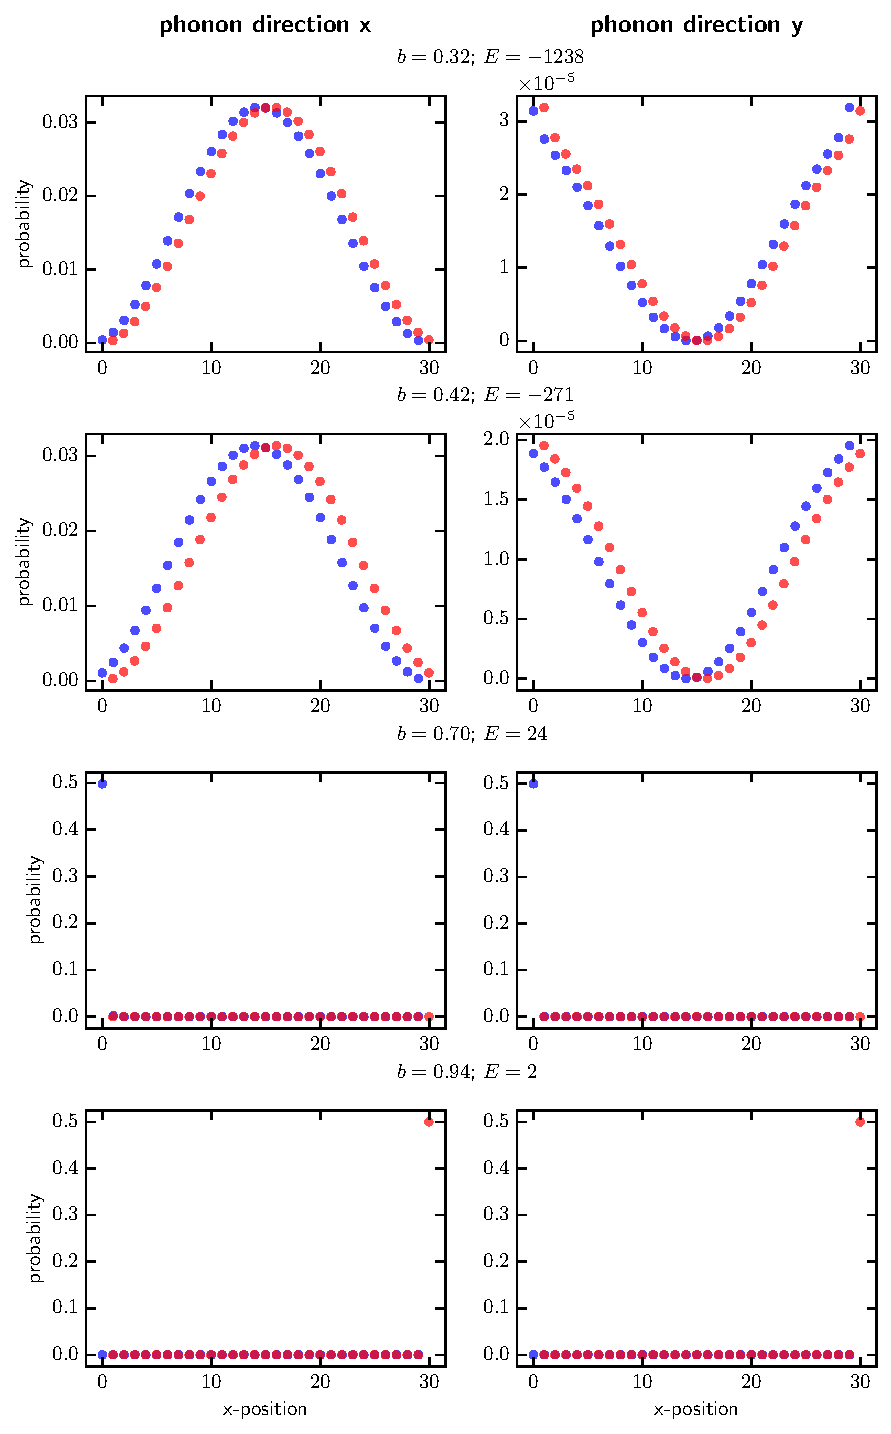
\includegraphics[]{pictures/aligned_dipoles_in_plane_zigzag_h0.2_eigenvecs.pdf}
\end{figure} 
\begin{figure}[H]
    \centering
    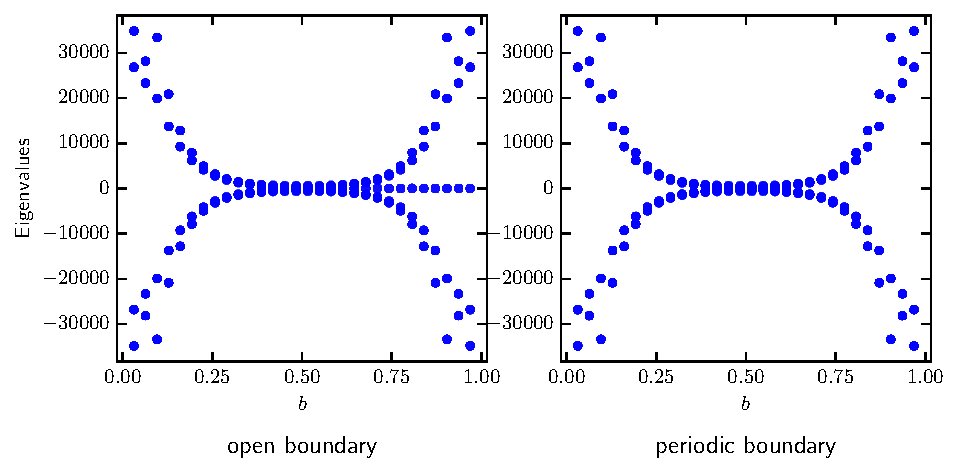
\includegraphics[]{pictures/aligned_dipole_in_plane_zigzag_spectrum_h0.2.pdf}
\end{figure} 
\begin{figure}[H]
    \centering
    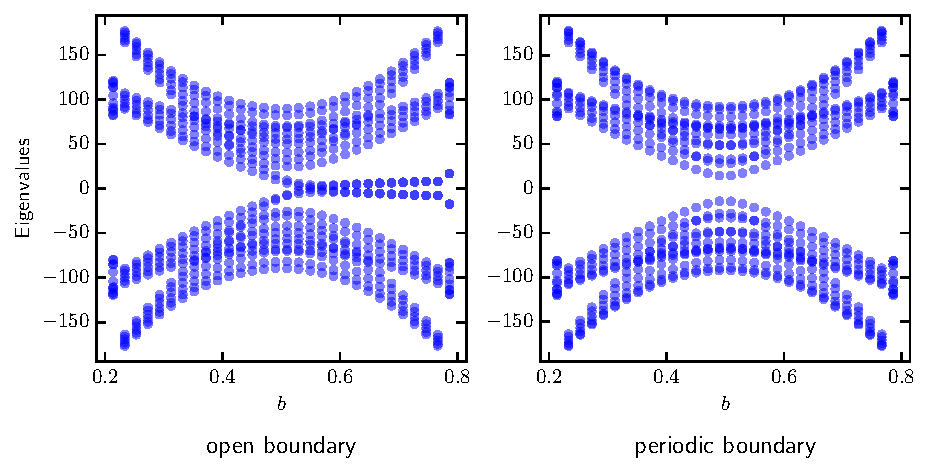
\includegraphics[]{pictures/aligned_dipole_in_plane_zigzag_spectrum_h0.6.pdf}
\end{figure} 
\begin{figure}[H]
    \centering
    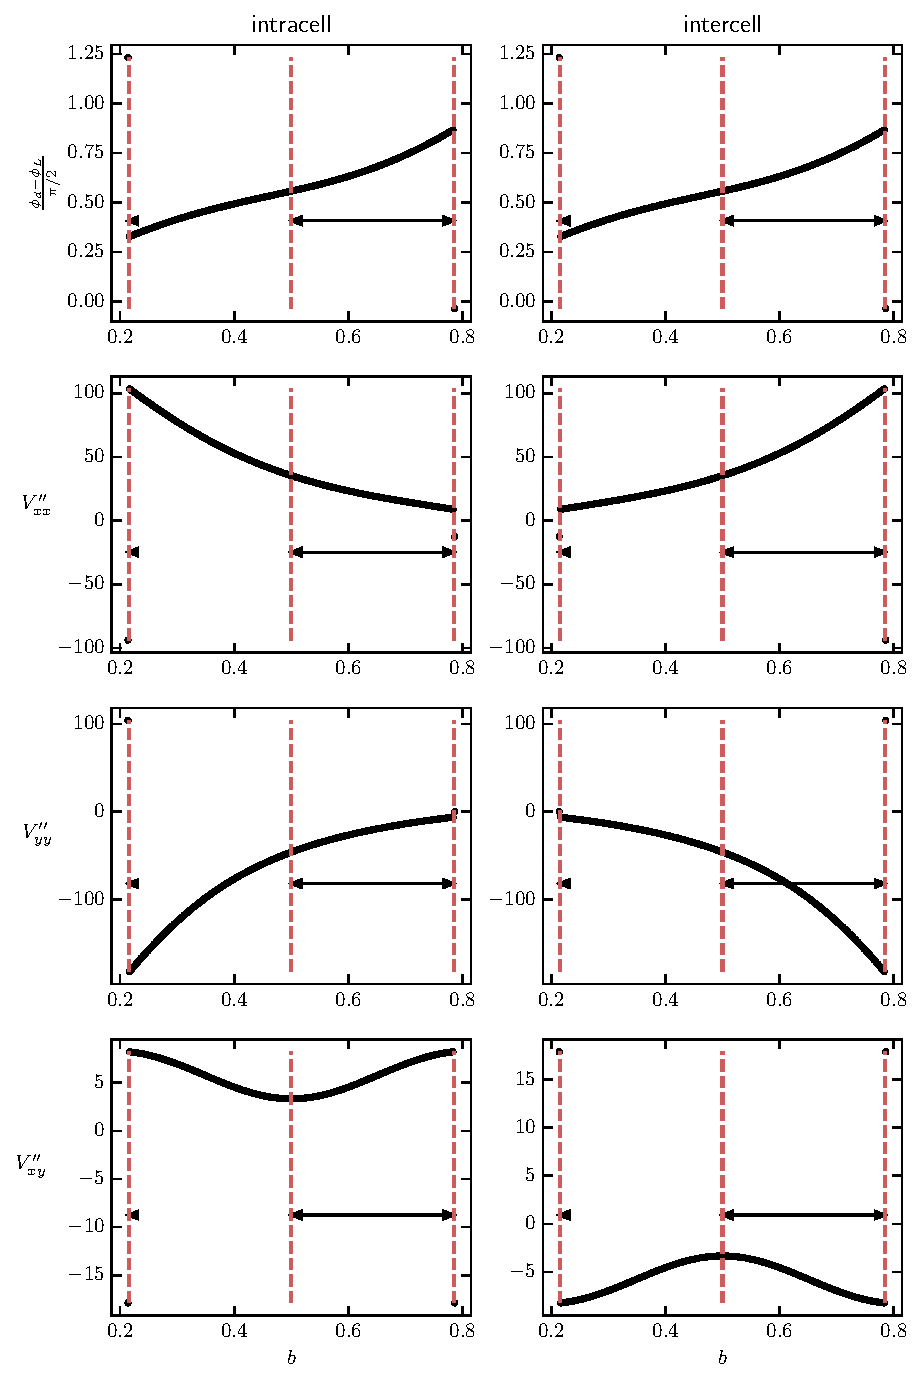
\includegraphics[]{pictures/aligned_dipoles_in_plane_zigzag_h0.6.pdf}
\end{figure} 
\begin{figure}[H]
    \centering
    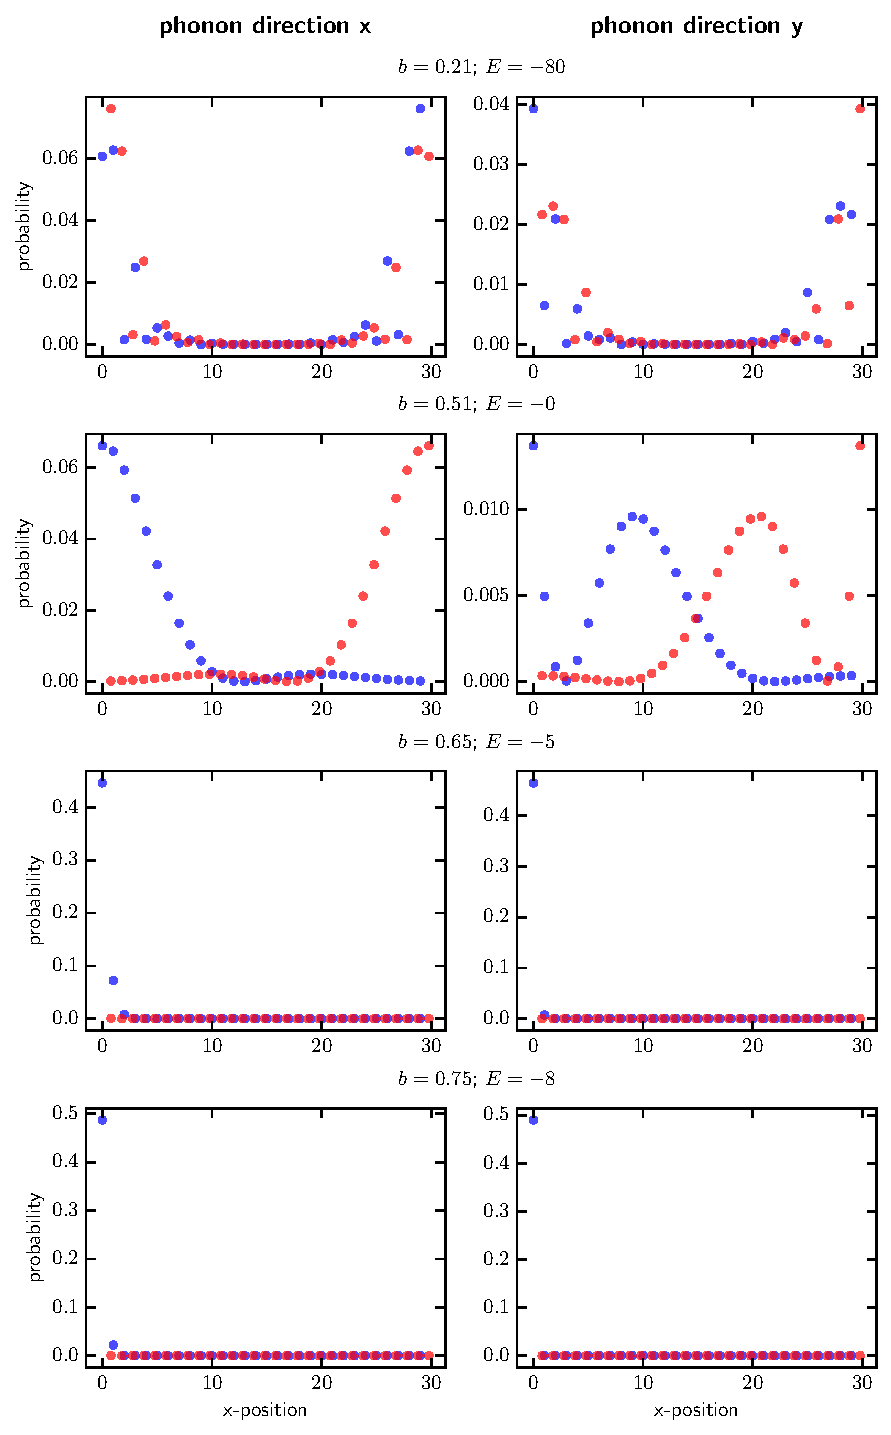
\includegraphics[]{pictures/aligned_dipoles_in_plane_zigzag_h0.6_eigenvecs.pdf}
\end{figure} 


\section{1D chain}
When allowing displacements in the 2-dimensional plane one can exploit the independence of the individual contributions to $H_k$, which implies that $X$ has to anti-commute with every contribution individually. Due to the results of \appref{appendix:symmetry} the only possible chiral symmetry in the case where $H_k^{A,A}$ is not identical zero is represented by the unitary
\begin{align*}
    S= \mathbb{1}\otimes\sigma_y
\end{align*}
It requires that the identity contribution in the second slot of the tensor product has to vanish. This can only be true if the $xx$ and $yy$ interaction have opposite signs.
% The first consequence is, that $H_k$ can not contain a term proportional to the identity. Thus $(H_k^{A,A})_0=0$ referring to the notation of \eqref{eq:xy-decomposition}. %The identity 
% % \begin{align*}
% %     \{\sigma_i\otimes\sigma_j,\sigma_n\otimes\sigma_m\}=\half\,\{\sigma_i,\sigma_n\}\otimes\{\sigma_j,\sigma_m\}
% % \end{align*}
% % which is derived in \secref{appendix:symmetry}, infers that possible contributions to an anti-commuting matrix $X$ contain
% % \begin{align*}
% %     \sigma
% % \end{align*}
% This term is determined by the interactions between sites of the same sublattice and modes of the same direction of displacement, i.e. $xx$ or $yy$, and the onsite term of $U$. The fact that $(H_k^{A,A})_0=0$ has to hold for all $k$ enforces the onsite term $U_{ii}^{\alpha,\alpha}=\sum_r\partial^2V_{dd}/\partial r_\alpha^2$ to be zero or have opposite sign for the two displacement directions. 
% Exploiting the high control of dipole traps in cold atom experiments one can tune the harmonic potential of each trap individually \cite{endresAtombyatomAssemblyDefectfree2016,youngHalfminutescaleAtomicCoherence2020}.
% Thus by fine tuning the trap frequencies at each site one can in principle cancel the onsite terms.

% At the same time one has to take into consideration that these conditions also have to be true at the borders of the chain, as in order for the bulk-boundary correspondence to be applicable both the infinite system as well as the open system have to respect the necessary symmetries. Thus if one wants to implement a system where the sum in the onsite potential vanishes, one has to make sure that the two parts of the sum, going to the right and to the left, vanish individually. Because of the vast decay of the interaction with $1/r^5$ I only considered up to next nearest neighbor interactions. In this case it was not possible to find a dipole orientation that meets the condition of vanishing onsite potential.
% Consequently I resort to the second possibility, to make interactions between $xx$ and $yy$ of opposite sign. 
Recall the dependence of the interaction of the direction of $\mathbf{r}$ and $\mathbf{d}$ in form of   
% Thus either the interactions inside a sublattice between the same direction have to vanish or the $xx$ and $yy$ interactions have to have opposite sign, allowing the $(H_k^{A,A})_0$ term to be non-zero. In the first case one has to tune the interactions between sites of the same sublattice to zero. But the onsite term $U_{ii}^{\alpha,\alpha}=\sum_r\partial^2V_{dd}/(\partial r_\alpha \partial r_\alpha)$ has to be considered as well. As the 

\begin{align*}
    c_{\alpha\beta}(\hat{\mathbf{r}}) &= \delta_{\alpha\beta}\left(-3 + 15\, (\hat{\mathbf{r}}\cdot \hat{\mathbf{d}})^2\right)- 6\,\hat{d}_\alpha \hat{d}_\beta +30\, \frac{\hat{d}_\alpha r_\beta + \hat{d}_\beta r_\alpha}{r}\,(\hat{\mathbf{r}}\cdot \hat{\mathbf{d}}) + 15\,\frac{r_\alpha r_\beta}{r^2} \left(1  - 7\, (\hat{\mathbf{r}}\cdot \hat{\mathbf{d}})^2\right)\\
    &= \delta_{\alpha\beta}\left(-3 + 15\, (\hat{\mathbf{r}}\cdot \hat{\mathbf{d}})^2\right) + A_{\alpha\beta}
\end{align*}
\begin{figure}[h]
    \hspace*{-2cm}
    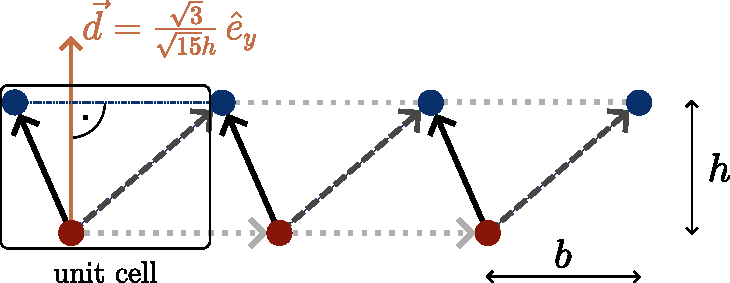
\includegraphics{pictures/chain_with_interaction_arrows2.pdf}
    \caption{\textbf{Zik-zak chain and dipole orientation.} Interactions up to next nearest neighbors are presented. The dipole is orientated in such a way that it is perpendicular to the connection vectors of nearest neighbor distances. Thus the scalar product with the dipole moment is the same for both the solid and the dashed vector.}
    \label{fig:chain and dipole orientation}
\end{figure}
% \hfill\newpage
In order for the interaction between atoms of relative distance $\mathbf{r}$ to vanish the following condition has to hold
\begin{align}\label{eq:opposite sign condition}
    c_{xx}(\hat{\mathbf{r}})&\overset{!}{=}-c_{yy}(\hat{\mathbf{r}})\\
    &=-6 + 30 \, (\hat{\mathbf{r}}\cdot \hat{\mathbf{d}})^2 + A_{xx}+A_{yy}\notag\\
    A_{xx}+A_{yy}&=- 6\,(\hat{d}_x^2+\hat{d}_y^2) +60\, \frac{\hat{d}_x r_x + \hat{d}_y r_y}{r}\,(\hat{\mathbf{r}}\cdot \hat{\mathbf{d}}) + 15\,\frac{r_x^2 + r_y^2}{r^2} \left(1  - 7\, (\hat{\mathbf{r}}\cdot \hat{\mathbf{d}})^2\right)\notag\\
    &= 9\,||d_{\parallel}||^2 - 3\cdot15\,(\hat{\mathbf{r}}\cdot \hat{\mathbf{d}})^2\notag\\
    \Rightarrow\quad (\hat{\mathbf{r}}\cdot \hat{\mathbf{d}}_{\parallel})^2&= \frac{3}{15}\notag
\end{align}
% and for the two different vectors ${\mathbf{r}}_1$ and ${\mathbf{r}}_2$ the interactions have different signs if
% \begin{gather*}
%     \frac{1}{r_1^5}\,c_{xx}(\hat{\mathbf{r}}_1)\overset{!}{=}-\frac{1}{r_2^5}\,c_{xx}(\hat{\mathbf{r}}_2)\quad\text{and}\quad \frac{1}{r_1^5}\,c_{yy}(\hat{\mathbf{r}}_1)\overset{!}{=}-\frac{1}{r_2^5}\,c_{yy}(\hat{\mathbf{r}}_2)\\
%     \Rightarrow\quad \frac{1}{r_1^5}\,\left[ 3 - 15\,(\hat{\mathbf{r}}_1\cdot \hat{\mathbf{d}})^2 \right] = -\frac{1}{r_2^5}\,\left[ 3 - 15\,(\hat{\mathbf{r}}_2\cdot \hat{\mathbf{d}})^2 \right]
% \end{gather*}

% \begin{align*}
% 3 - 15 d_x^2 &= -\frac{1}{r^5} \left[ 3 - \frac{15}{r^2}\, \left( r_x^2 d_x^2 + r_y^2 d_y^2 + 2 r_x r_y d_x d_y \right) \right] \\[1ex]
% 0 &= 3 r^5 + 3 - 15 \left( r^5 + \frac{r_x^2}{r^2} \right) d_x^2 - 15 \frac{r_y^2}{r^2} d_y^2 + 30 \frac{r_x r_y}{r^2} d_x d_y
% \end{align*}
This condition can only be satisfied when all vectors lie on a straight line. Picturing the zik-zak chain implementation of the system as depicted in \figref{fig:chain and dipole orientation} one realizes that this is not possible if one encounters bot interactions between  and within the sublattices.
However, the restriction to only nearest neighbor interactions lets the coupling only take place between sublattices and one can choose the dipole moment in $y$ direction to satisfy \eqref{eq:opposite sign condition} as in \figref{fig:chain and dipole orientation}. In this case the model only contains four different coupling parameters, $V_x$, $V_{xy}$ for interactions within the unit cell and $W_x$, $W_{xy}$ for interactions between unit cells. One can write down the contributions to the Hamiltonian as
\begin{align*}
    H_k^{A,A}&=\begin{pmatrix}
        V_x + W_x & V_{xy} + W_{xy}\\
        V_{xy} + W_{xy} & -V_x - W_x
    \end{pmatrix}=(V_x + W_x)\,\sigma_z+(V_{xy} + W_{xy})\,\sigma_x\\\\
    H_k^{A,B} &= \begin{pmatrix}
        V_x + W_x \, e^{-ika}& V_{xy} + W_{xy}\, e^{-ika}\\
        V_{xy} + W_{xy} \, e^{-ika}& -V_x - W_x\, e^{-ika}
    \end{pmatrix}=\left(V_x + W_x\, e^{-ika}\right)\,\sigma_z+\left(V_{xy} + W_{xy}\, e^{-ika}\right)\,\sigma_x
\end{align*}
% $H_k$ is still irreducible (see \secref{appendix:symmetry}). Thus the anti-commutation property with the matrix 
% \begin{align*}
%     S= \mathbb{1}\otimes\sigma_y
% \end{align*}
% is the unique chiral symmetry of the system. 
Transforming to the basis where $S=\sigma_z\otimes\mathbb{1}$ the Hamiltonian takes the form
\begin{align*}
    H_k&=\begin{pmatrix}
        0&h\\
        h^\dagger&0
    \end{pmatrix}\\
    \text{with}\quad h&= \begin{pmatrix}i\,(V_{xy}+W_{xy})-(V_x+W_x)  & i\,\left(V_{xy} + W_{xy}\, e^{-ika}\right)-\left(V_x + W_x\, e^{-ika}\right)\\
        i\,\left(V_{xy} + W_{xy}\, e^{ika}\right)-\left(V_x + W_x\, e^{ika}\right) & i\,(V_{xy}+W_{xy})-(V_x+W_x)
    \end{pmatrix}
\end{align*}
This can be written in shorter and clearer form as
\begin{align*}
    h&=\begin{pmatrix}
        a & b+c\,e^{-ika}\\
        b+c\,e^{ika}& a
    \end{pmatrix}\quad a,b,c\in\mathbb{C}
\end{align*}
From this the eigenvalues $\lambda_\pm$ can be calculated as
\begin{align*}
    \lambda_\pm&= a\pm\sqrt{b^2+c^2+2bc\,\cos(ka)}
\end{align*}
Since $a$ is constant the only winding can come from the square root expression. As the discriminant is, however, of the form $r+s\,t$ with $r,s\in\mathbb{C}$ and $t\in[0,1]$ the square root cannot describe a closed curve in the complex plain. Hence this implementation of chiral symmetry does not exhibit topologically non-trivial phases.\\\\
In order to have a qualitatively different disorder, one has to make the $H_k^{A,A}$ term vanish. Since one cannot choose the dipole in such a way that the $xx$, $yy$ and $xy$ interaction of one distance vanish at the same time, one has to assume nearest neighbor interactions only. In this scenario one is still left with the onside terms of $U$. Exploiting the high control of dipole traps in cold atom experiments one can tune the harmonic potential of each trap individually \cite{endresAtombyatomAssemblyDefectfree2016,youngHalfminutescaleAtomicCoherence2020}.
Thus by fine tuning the trap frequencies at each site one can in principle cancel the onsite terms corresponding to $xx$ and $yy$ interactions. The interaction between different direction, however, is still present after this step and has to be tuned to zero via the geometry of the lattice and the dipole orientation. This decouples the two direction completely from each other leading to a mere coexistence of two models. It has to be noted that the open system with boundaries has to satisfy the same symmetries as the infinite system in order for the bulk-boundary correspondence to hold. Hence it is not possible to tune the sum in $U_{ii}^{xy}=\sum_r\partial^2V_{dd}/\partial r_x\partial r_y$ to zero for every site of the open system without forcing every summand to zero. 
After decoupling into one model for each direction of displacement, it is, however, possible to observe both models in different topological phases at the same time, as indicated by \figref{fig:topological phases 1D}.
\begin{addmargin}[2em]{2em} % [left margin]{right margin}
\small \textbf{Note:} The value of the derivative of the dipole-dipole interaction on the unit circle is only dependent on two properties. On the one hand the dipole-dipole interaction is only dependent on the angle between dipole and distance vector. The derivative on the other hand is additionally dependent on the direction of derivation, thus by the choice of the coordinate frame. If the frame is rotated by the angle $\varphi$ around the $z$-axis, one can write the old variables as functions of the new ones.
\begin{align*}
    r_x&= \cos\varphi\,r_x' + \sin\varphi\,r_y'\\
    r_y&= -\sin\varphi\,r_x' + \cos\varphi\,r_y'
\end{align*}
From this expression one can write the derivations into the new $x$- and $y$-directions.
\begin{align*}
    \frac{\partial V_{dd}}{\partial r_x'}&=  \frac{\partial V_{dd}}{\partial r_x}\,\cos\varphi - \frac{\partial V_{dd}}{\partial r_y}\,\sin\varphi\\
    \frac{\partial^2 V_{dd}}{(\partial r_x')^2}&= \cos^2\varphi\,\frac{\partial^2 V_{dd}}{\partial r_x^2} - 2\,\cos\varphi\sin\varphi\,\frac{\partial^2 V_{dd}}{\partial r_x\partial r_y}+\sin^2\varphi\,\frac{\partial^2 V_{dd}}{\partial r_y^2}\\
    % 
    \frac{\partial^2 V_{dd}}{(\partial r_y')^2}&= \sin^2\varphi\,\frac{\partial^2 V_{dd}}{\partial r_x^2} + 2\,\cos\varphi\sin\varphi\,\frac{\partial^2 V_{dd}}{\partial r_x\partial r_y}+\cos^2\varphi\,\frac{\partial^2 V_{dd}}{\partial r_y^2}\\
    %
    \frac{\partial^2 V_{dd}}{\partial r_x'\partial r_y'}&= \cos\varphi\sin\varphi\,\frac{\partial^2 V_{dd}}{\partial r_x^2} - \left(\cos^2\varphi-\sin^2\varphi\right)\,\frac{\partial^2 V_{dd}}{\partial r_x\partial r_y}-\cos\varphi\sin\varphi\,\frac{\partial^2 V_{dd}}{\partial r_y^2}\\
\end{align*}
All three derivatives in the new frame can only be zero if they where already zero in the old reference frame. As it is not possible to find a dipole orientation that makes this happen for the direction $\hat{e}_x$. It is not possible to find another orientation of the distance vector such that all second derivatives would vanish.
\end{addmargin}
\begin{figure}[h]
    \hspace*{-2cm}
    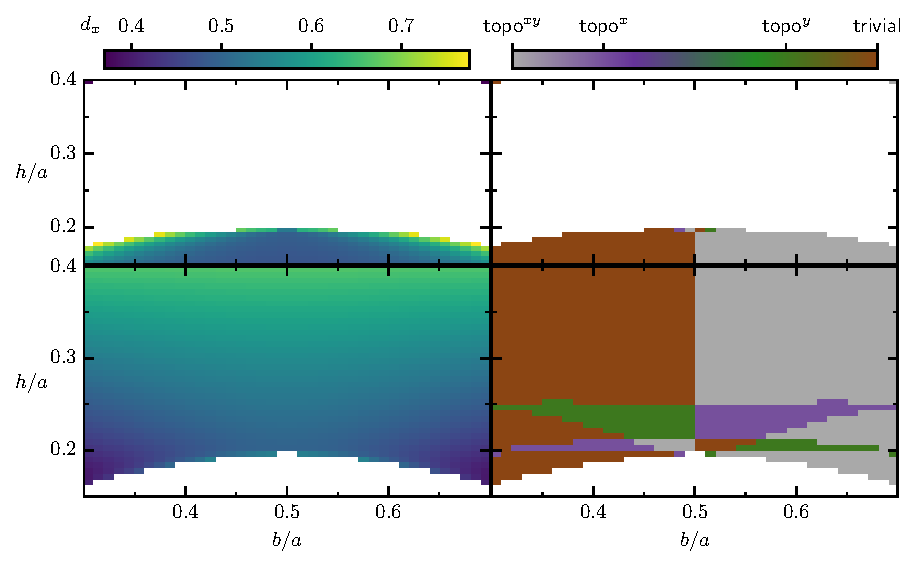
\includegraphics{pictures/topological_phases_decoupled_2D.pdf}
    \caption{\textbf{Topological phase diagram.} There are up to four possible dipole orientations that decouple $x$ and $y$-directions. Two of them are shown on the left panels by depicting the $x$-component of the dipole. White space indicates here that there were no appropriate dipoles found. On the right side of the panel the topological phases are depicted. It is shown, whether a topological phase arises for the $x$, $y$ or both directions, or if the system exhibits a topologically trivial phase.}
    \label{fig:topological phases 1D}
\end{figure}
A different approach to decoupling the two directions of displacement $x$ and $y$, is by choosing different trap frequencies along each direction (see \secref{sec:dipole traps}). If one can still ensure $|\omega_x-\omega_y|\gg|U|\ll\omega_x,\,\omega_y$, the two direction of displacement are decoupled as well, since transfer between the $x$ and $y$-mode are suppressed. In this case one still has free choice over the dipole orientation. Focussing in the following only on one direction, one receives a full one-dimensional model with one mode per site. Eliminating the onsite potential with the help of the trap frequencies, this system can be mapped to an extended SSH-model. The only requirement left for this mapping is the vanishing of interactions within the same sublattice. This can be eliminated by choosing an appropriate dipole orientation, i.e. $d_x=\pm1/\sqrt{3}$.


